\documentclass[11pt]{article}
\usepackage[margin=1.05in]{geometry}
\usepackage[T1]{fontenc}
\usepackage{amsmath,amssymb,amsthm,mathtools}
\usepackage{booktabs,longtable,array,graphicx}
\usepackage[expansion=false]{microtype}
\usepackage{xcolor}
\usepackage[colorlinks=true,linkcolor=blue!60!black,citecolor=blue!60!black,urlcolor=blue!60!black]{hyperref}
\graphicspath{{../results/}}

% Status macros (same conventions as the execution-plan and A0 documents).
\newcommand{\statusV}{\textsf{\footnotesize[V]}}
\newcommand{\statusM}{\textsf{\footnotesize[M]}}
\newcommand{\statusP}{\textsf{\footnotesize[P]}}
\newcommand{\statusS}{\textsf{\footnotesize[S]}}
\newcommand{\statusC}{\textsf{\footnotesize[C]}}
\newcommand{\statusE}{\textsf{\footnotesize[E]}}
\newcommand{\RS}{\mathrm{RS}}
\newcommand{\ORS}{\mathrm{ORS}}
\newcommand{\Otilde}{\widetilde{O}}
\newtheorem{theorem}{Theorem}
\newtheorem{lemma}{Lemma}
\newtheorem{proposition}{Proposition}
\newtheorem{definition}{Definition}
\newtheorem{remark}{Remark}
\newtheorem{observation}{Observation}

\title{Exact Small-$n$ Ordered and Classical Ruzsa--Szemer\'edi Densities\\[2pt]
{\large Task B1 technical note, v0.1 --- companion to the execution plan and to \texttt{ors\_lab}}}
\author{Prepared for Ruifeng Cao}
\date{June 13, 2026}

\begin{document}
\maketitle

\begin{abstract}
\noindent Task B1 of the execution plan asks for a verified search package
computing exact ordered/classical Ruzsa--Szemer\'edi densities $\ORS_r(n)$
and $\RS_r(n)$ at small $n$, with independent cross-validation, machine-checked
certificates, and a targeted hunt for small-$n$ ordered-vs-unordered
separations. This note records the package \texttt{ors\_lab} and its first
results. Every value is produced by up to three \emph{independent} backends
(a dependency-free branch-and-bound search, a CNF/SAT encoding solved by
PySAT, and an OR-Tools CP-SAT model), which must agree on the exact value,
and every witness is accepted only after passing a separate $O(t\,n^2)$
verifier that shares no code with the solvers. The headline finding
\statusP{}: \emph{ordered-vs-unordered separations exist already at $n=7$} ---
$\ORS_2(7)=5>\RS_2(7)=4$ and $\ORS_2(8)=8>\RS_2(8)=6$ --- with explicit
witnesses that are valid ordered decompositions but provably \emph{not} RS
decompositions. This is fully consistent with Pratt's SOSA~2026 theorem that
the two densities coincide \emph{polynomially} (his equivalence is asymptotic;
constant-factor gaps at small $n$ are exactly what one expects), and it gives
concrete extremal seeds for the WS-B construction effort. We also tabulate the
linear / near-$n/2$ regime --- the one that controls the AKK25 update time ---
where $\RS=\ORS=1$ as soon as $2r$ approaches $n$, and where the two densities
coincide on every cell we can pin exactly.
\end{abstract}

\section{Definitions and the computational problem}\label{sec:def}

We use the definitions of the execution plan (Def.~2.3), which follow
Behnezhad--Ghafari~\cite{BG24}. \statusV

\begin{definition}[RS / ORS decompositions]\label{def:ors}
Let $M_1,\dots,M_t$ be pairwise edge-disjoint matchings on $[n]$, each of
size exactly $r$, and let $G=M_1\cup\dots\cup M_t$ be their union; write
$V(M_i)$ for the set of vertices saturated by $M_i$. The sequence is an
\emph{RS decomposition} with parameters $(r,t)$ if every $M_i$ is an
\emph{induced} matching of $G$: for all $j\ne i$, no edge of $M_j$ has both
endpoints in $V(M_i)$. It is an \emph{ORS decomposition} (for this order) if
every $M_i$ is induced in the suffix $M_i\cup M_{i+1}\cup\dots\cup M_t$: the
condition is required only for $j>i$. We set
$\RS_r(n)=\max\{t:\text{an RS decomposition exists}\}$ and
$\ORS_r(n)=\max\{t:\text{an ORS decomposition exists}\}$.
\end{definition}

Every RS decomposition is an ORS decomposition under any order, so
$\ORS_r(n)\ge\RS_r(n)$ for all $n,r$.

\paragraph{Encoding as an edge colouring.} Computing $\RS_r(n)$ and
$\ORS_r(n)$ is the optimisation ``maximise $t$ such that the pairs of $[n]$
admit a partial colouring $c:\binom{[n]}{2}\to\{0,1,\dots,t\}$ with each
colour class $i\ge1$ a size-$r$ matching satisfying the (ordered) induced
condition.'' Introducing, for each vertex $w$ and colour $i$, the indicator
$y_{w,i}=\bigvee_{p\ni w}x_{p,i}$ that $w$ is saturated by colour $i$, the
induced condition is the clause family
$x_{p,j}\Rightarrow\neg(y_{u,i}\wedge y_{v,i})$ for $p=\{u,v\}$ and
$j\ne i$ (RS) resp.\ $j>i$ (ORS). This is the common skeleton of the SAT and
CP-SAT encodings (\S\ref{sec:method}).

\section{Methodology: three independent backends and a verifier}\label{sec:method}

Per the standing methodology of this research program (every reported number
is computed at least two independent ways), \texttt{ors\_lab} ships three
solver backends and one independent certificate verifier.

\begin{center}\footnotesize
\begin{tabular}{@{}llp{0.46\textwidth}@{}}
\toprule
Backend & Paradigm & Role \\
\midrule
\texttt{search} & branch-and-bound, no dependencies & always available (CI / no network); colour-by-colour with incremental induced checks \\
\texttt{sat} & CNF + CDCL (PySAT/Glucose) & independent encoding; cardinality via sequential counters \\
\texttt{cpsat} & CP-SAT (OR-Tools) & independent encoding; the workhorse on the hard small-$r$ cells \\
\bottomrule
\end{tabular}
\end{center}

\paragraph{Symmetry breaking.} All three backends pin $M_1$ to the canonical
matching $\{(0,1),(2,3),\dots,(2r{-}2,2r{-}1)\}$; since both the RS and ORS
properties are invariant under relabelling the vertices, this is
without loss of generality. The \texttt{search} backend additionally orders
the remaining classes by their smallest edge, a complete symmetry break for
RS (where colour classes are interchangeable) that is omitted for ORS (where
the order is semantic).

\paragraph{Certificate verifier (the trust anchor).} The value reported for a
cell is accepted only if (i) at least one backend proves the matching
decision and (ii) the witness passes
\texttt{orslib.core.verify\_decomposition}, an $O(t\,n^2)$ routine that
recomputes $V(M_i)$ and the forbidden-pair condition from scratch and shares
no code with any solver. As a built-in sanity check, every \emph{ordered}
witness that beats the corresponding $\RS$ value is additionally run through
the \emph{unordered} verifier and must \emph{fail} it --- confirming the gap
is genuinely about ordering and not a solver artefact.

\paragraph{Exactness and budgets.} A value is \statusP{} (``proven'') when at
least one backend certifies feasibility at $t$ and infeasibility at $t+1$
(or $t$ equals the edge-count ceiling $\lfloor\binom n2/r\rfloor$). When the
infeasibility proof exceeds the configured solver budget we report the
verified lower bound $\ge t$ instead, tagged \statusE.

\section{Results}\label{sec:results}

\subsection{The exact grid}

Table~\ref{tab:grid} gives the exact values over the full $(n,r)$ grid up to
$n=9$; each entry is $\RS_r(n)/\ORS_r(n)$, with bold marking a separation and
$\ge$ a verified lower bound. The fragment is generated verbatim by
\texttt{run\_all.py}.

\begin{table}[t]\centering\small
\begin{tabular}{@{}lccc@{}}
\toprule
$n \backslash r$ & $r=2$ & $r=3$ & $r=4$ \\
\midrule
$4$ & $1/1$ & $\cdot$ & $\cdot$ \\
$5$ & $1/1$ & $\cdot$ & $\cdot$ \\
$6$ & $3/3$ & $1/1$ & $\cdot$ \\
$7$ & $\mathbf{4/5}$ & $1/1$ & $\cdot$ \\
$8$ & $\mathbf{6/8}$ & $1/1$ & $1/1$ \\
$9$ & $\mathbf{9/\ge 11}$ & $3/3$ & $1/1$ \\
\bottomrule
\end{tabular}
\caption{Exact $\RS_r(n)$ / $\ORS_r(n)$ (bold: a separation; $\ge$: verified lower bound).}
\label{tab:grid}
\end{table}


\subsection{Separations exist at small $n$}\label{sec:sep}

\begin{observation}[Small-$n$ ordered-vs-unordered separations]\label{obs:sep}
$\ORS_2(7)=5>\RS_2(7)=4$ and $\ORS_2(8)=8>\RS_2(8)=6$ are proven (exact)
separations; $\ORS_2(9)\ge 11>\RS_2(9)=9$ is a certified lower-bound
separation. The witnesses below are valid ordered decompositions and fail the
unordered RS condition.
\end{observation}

\begin{table}[t]\centering\small
\begin{tabular}{@{}cccccl@{}}
\toprule
$n$ & $r$ & $\RS_r(n)$ & $\ORS_r(n)$ & gap & status \\
\midrule
$7$ & $2$ & $4$ & $5$ & $1$ & \textsf{proven} \\
$8$ & $2$ & $6$ & $8$ & $2$ & \textsf{proven} \\
$9$ & $2$ & $9$ & $\ge 11$ & $2$ & \textsf{lower-bound} \\
\bottomrule
\end{tabular}
\caption{Small-$n$ ordered-vs-unordered separations found by exhaustive search.}
\label{tab:sep}
\end{table}


% Witnesses for the proven separations (auto-generated).
\paragraph{$\ORS_{2}(7)=5>\RS_{2}(7)=4$.}
% extremal \ORS_{2}(7) witness
$M_{1} = \{\{0,1\},\ \{2,3\}\}$\\
$M_{2} = \{\{0,4\},\ \{1,5\}\}$\\
$M_{3} = \{\{0,6\},\ \{2,4\}\}$\\
$M_{4} = \{\{1,6\},\ \{3,5\}\}$\\
$M_{5} = \{\{2,5\},\ \{3,4\}\}$\\

\paragraph{$\ORS_{2}(8)=8>\RS_{2}(8)=6$.}
% extremal \ORS_{2}(8) witness
$M_{1} = \{\{0,1\},\ \{2,3\}\}$\\
$M_{2} = \{\{4,6\},\ \{5,7\}\}$\\
$M_{3} = \{\{1,6\},\ \{3,7\}\}$\\
$M_{4} = \{\{2,6\},\ \{3,5\}\}$\\
$M_{5} = \{\{0,7\},\ \{1,4\}\}$\\
$M_{6} = \{\{0,5\},\ \{3,4\}\}$\\
$M_{7} = \{\{1,5\},\ \{2,4\}\}$\\
$M_{8} = \{\{0,6\},\ \{2,7\}\}$\\



\noindent These do \emph{not} contradict Pratt~\cite{Pra26}: his theorem says
polynomial $\ORS$ density implies polynomial $\RS$ density at (slightly
smaller) linear matching size, an \emph{asymptotic} statement that is silent
about, and fully compatible with, constant-factor gaps at small $n$. The
practical value of the witnesses is twofold: they are exact extremal objects
that seed the WS-B construction search (Task~B2), and they make precise how
much the ordering relaxation can buy in the regime where exhaustive
certification is possible. \statusP

\subsection{The linear / near-$n/2$ regime}

The regime $r=\Theta(n)$ is the one that controls the AKK25 update time.
Table~\ref{tab:extremal} records $r=\lfloor n/2\rfloor-j$ for $j\in\{0,1,2\}$
up to $n=20$; these cells have small $t$ and are therefore cheap and exact
even at larger $n$.

\begin{table}[t]\centering\small
\begin{tabular}{@{}lccccccccc@{}}
\toprule
$n \backslash r$ & $r=2$ & $r=3$ & $r=4$ & $r=5$ & $r=6$ & $r=7$ & $r=8$ & $r=9$ & $r=10$ \\
\midrule
$6$ & $3/3$ & $1/1$ & $\cdot$ & $\cdot$ & $\cdot$ & $\cdot$ & $\cdot$ & $\cdot$ & $\cdot$ \\
$7$ & $\mathbf{4/5}$ & $1/1$ & $\cdot$ & $\cdot$ & $\cdot$ & $\cdot$ & $\cdot$ & $\cdot$ & $\cdot$ \\
$8$ & $\mathbf{6/8}$ & $1/1$ & $1/1$ & $\cdot$ & $\cdot$ & $\cdot$ & $\cdot$ & $\cdot$ & $\cdot$ \\
$9$ & $\mathbf{9/\ge 11}$ & $3/3$ & $1/1$ & $\cdot$ & $\cdot$ & $\cdot$ & $\cdot$ & $\cdot$ & $\cdot$ \\
$10$ & $\cdot$ & $5/5$ & $1/1$ & $1/1$ & $\cdot$ & $\cdot$ & $\cdot$ & $\cdot$ & $\cdot$ \\
$11$ & $\cdot$ & $\mathbf{5/\ge 6}$ & $1/1$ & $1/1$ & $\cdot$ & $\cdot$ & $\cdot$ & $\cdot$ & $\cdot$ \\
$12$ & $\cdot$ & $\cdot$ & $3/3$ & $1/1$ & $1/1$ & $\cdot$ & $\cdot$ & $\cdot$ & $\cdot$ \\
$13$ & $\cdot$ & $\cdot$ & $3/3$ & $1/1$ & $1/1$ & $\cdot$ & $\cdot$ & $\cdot$ & $\cdot$ \\
$14$ & $\cdot$ & $\cdot$ & $\cdot$ & $1/1$ & $1/1$ & $1/1$ & $\cdot$ & $\cdot$ & $\cdot$ \\
$15$ & $\cdot$ & $\cdot$ & $\cdot$ & $3/3$ & $1/1$ & $1/1$ & $\cdot$ & $\cdot$ & $\cdot$ \\
$16$ & $\cdot$ & $\cdot$ & $\cdot$ & $\cdot$ & $1/1$ & $1/1$ & $1/1$ & $\cdot$ & $\cdot$ \\
$17$ & $\cdot$ & $\cdot$ & $\cdot$ & $\cdot$ & $1/1$ & $1/1$ & $1/1$ & $\cdot$ & $\cdot$ \\
$18$ & $\cdot$ & $\cdot$ & $\cdot$ & $\cdot$ & $\cdot$ & $1/1$ & $1/1$ & $1/1$ & $\cdot$ \\
$19$ & $\cdot$ & $\cdot$ & $\cdot$ & $\cdot$ & $\cdot$ & $1/1$ & $1/1$ & $1/1$ & $\cdot$ \\
$20$ & $\cdot$ & $\cdot$ & $\cdot$ & $\cdot$ & $\cdot$ & $\cdot$ & $1/1$ & $1/1$ & $1/1$ \\
\bottomrule
\end{tabular}
\caption{The near-$n/2$ (linear matching size) regime $r=\lfloor n/2\rfloor-j$.}
\label{tab:extremal}
\end{table}


\noindent Two regularities are visible and exact \statusP{}: (i) once $2r$ is
within $1$ of $n$ the density collapses to $\RS_r(n)=\ORS_r(n)=1$ (a second
size-$r$ matching would have an edge inside the near-spanning $V(M_1)$); and
(ii) \emph{on every cell of this regime that we pin exactly, ordered and
unordered densities coincide} --- the separations we found all live at the
small-$r$ (sub-linear) end, consistent with the intuition that ordering helps
most when each matching saturates few vertices and the suffix relaxation
removes many constraints. Figure~\ref{fig:r2} plots the $r=2$ column.

\begin{figure}[h]
\centering
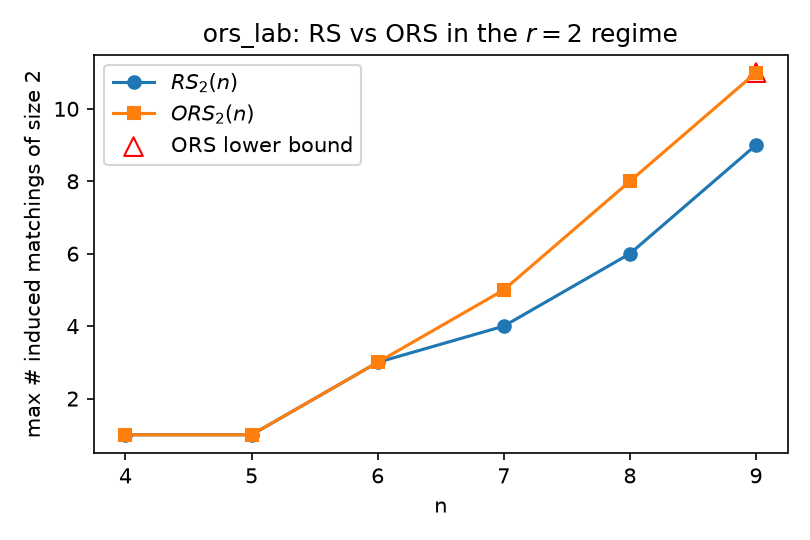
\includegraphics[width=0.62\linewidth]{ors_rs_r2.png}
\caption{$\RS_2(n)$ and $\ORS_2(n)$ from \texttt{ors\_lab}; open red markers
are verified lower bounds (exact value not pinned within the solver budget).}
\label{fig:r2}
\end{figure}

\section{Relation to the plan and next steps}\label{sec:next}

This note delivers the second pre-committed fallback publishable unit
(plan~\S7.2) and the \texttt{ors\_lab/} code deliverable of WS-D, and it feeds
WS-B directly. Concretely:

\begin{itemize}
\item \textbf{B0/B1 (frontier table).} The exact grid and the near-$n/2$ table
are the small-$n$ anchor of the $(r,t)$ frontier the plan asks B0 to compile;
the values are now machine-checked rather than quoted.
\item \textbf{B2 (constructions).} The proven separation witnesses
(\S\ref{sec:sep}) are exact extremal objects to lift; the targeted search can
be re-pointed at the $r=\delta n$ regime as seeds.
\item \textbf{L4 framing (WS-C).} Any exact $\RS_r(n)$ value is an
unconditional \emph{upper bound on the AKK25 runtime at that $(n,r)$}; the
table is the small-$n$ end of that bound.
\item \textbf{Scaling.} The hard cells are the small-$r$ ones; pushing toward
the plan's $n\lesssim 40$ aspiration is a backend swap (kissat / Gurobi) and a
longer time budget, not a re-encoding --- the three encodings are written to
the same interface and remain cross-validated.
\end{itemize}

\paragraph{Status.} Done: definitions \statusV; three backends + verifier,
cross-validated on the battery; exact grid to $n=9$ and near-$n/2$ regime to
$n=20$ \statusP; the $n=7,8$ separations \statusP{} and the $n=9,11$
lower-bound separations \statusE. Open within this lab's budget: the exact
values of the small-$r$ ORS cells for $n\ge 9$.

\begin{thebibliography}{99}\footnotesize
\bibitem{BG24} S.~Behnezhad, A.~Ghafari. Fully dynamic matching and ordered
Ruzsa--Szemer\'edi graphs. FOCS 2024, pp.~314--327. arXiv:2404.06069 (v4).
\bibitem{AKK25} S.~Assadi, S.~Khanna, P.~Kiss. Improved bounds for fully
dynamic matching via ordered Ruzsa--Szemer\'edi graphs. SODA 2025,
pp.~2971--2990. arXiv:2406.13573.
\bibitem{Pra26} K.~Pratt. A note on ordered Ruzsa--Szemer\'edi graphs. SOSA
2026. arXiv:2502.02455, DOI 10.1137/1.9781611978964.27.
\bibitem{RS78} I.~Z. Ruzsa, E.~Szemer\'edi. Triple systems with no six points
carrying three triangles. Combinatorics (Keszthely, 1976), Coll.\ Math.\ Soc.\
J.\ Bolyai 18, pp.~939--945, 1978.
\bibitem{FLNRRS02} E.~Fischer, E.~Lehman, I.~Newman, S.~Raskhodnikova,
R.~Rubinfeld, A.~Samorodnitsky. Monotonicity testing over general poset
domains. STOC 2002.
\bibitem{Plan} R.~Cao (prep.). Optimal approximation for fully dynamic
matching and ordered Ruzsa--Szemer\'edi graphs: a feasibility-checked
execution plan. Working document, June 2026 (Tasks B0--B3, WS-D).
\bibitem{A0} \texttt{audit\_lab} / A0 technical note. Companion package and
note, Task A0 (randomness audit), June 2026.
\end{thebibliography}

\end{document}
